\section{Massively Learning Activities II - Migration Deployment} \label{section: MLA2}
The System Development Life-cycle (SDLC) is a project management model that defines different stages that are necessary to bring a project from conception to deployment and later maintenance. 

The SDLC model consists of several phases: planning, research, design, implementation, testing \& integration, and maintenance. It provides a systematic approach to system development that helps ensure that system is built efficiently with minimal risk.

We explore the logistics of configuring a multi-tenant environment by documenting the entire project management process, inspired by the System Development Life-Cycle framework.  Massively Learning Activities will follow a similar variation of the SDLC project management model where each SDLC stage will correspond to a subsection in this chapter. 

\begin{figure}[H]
    \centering
    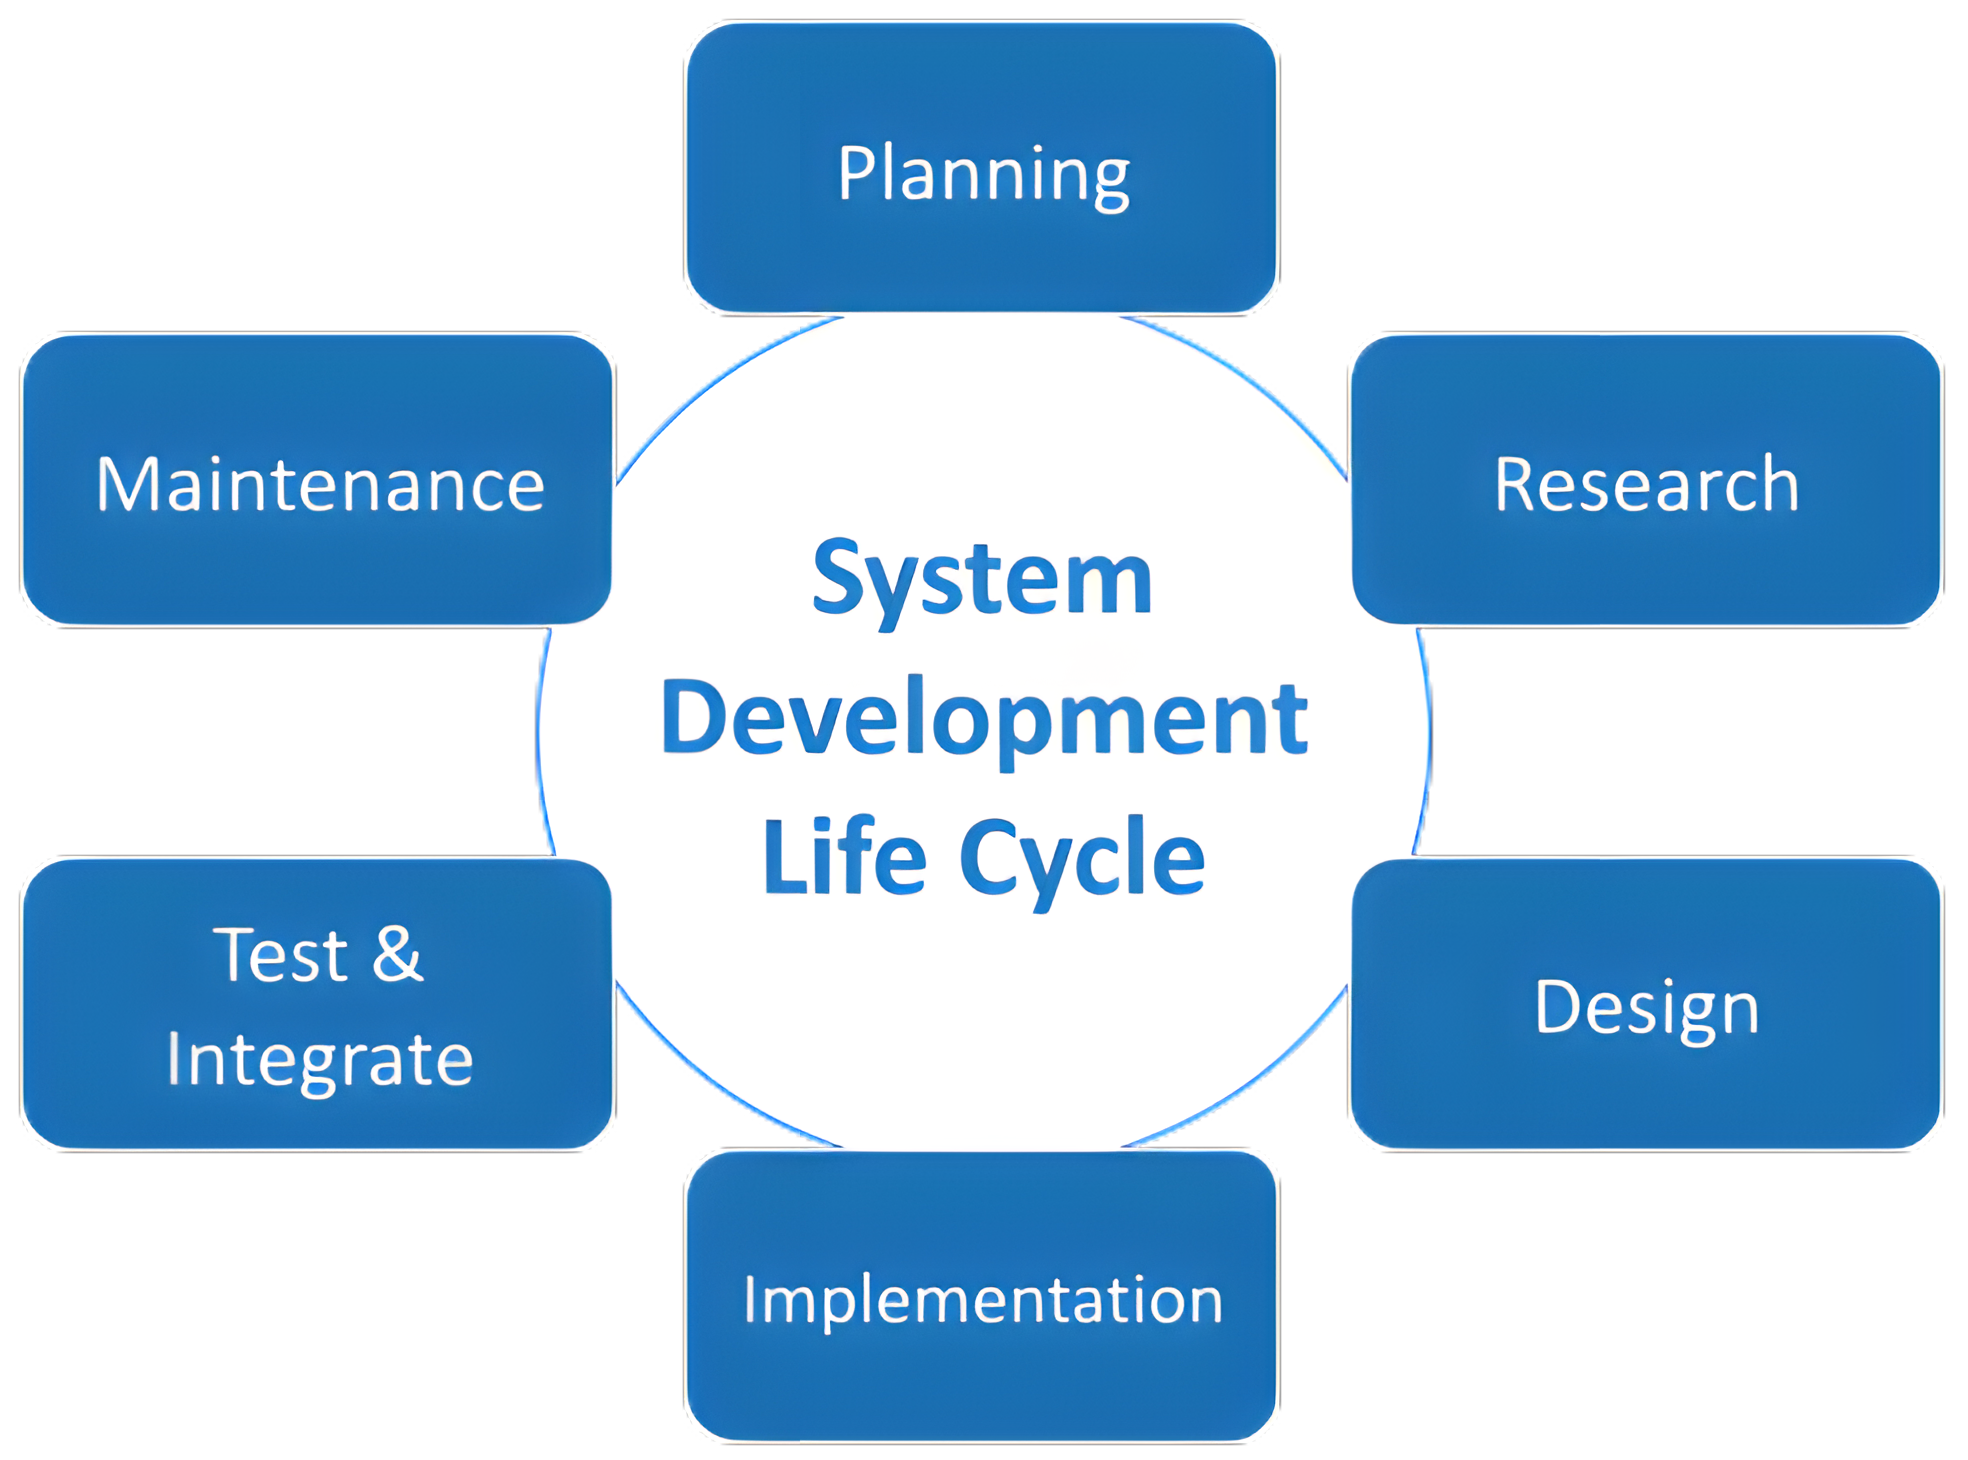
\includegraphics[scale = 0.175]{images/SDLC.png}
    \caption{System Development Life-Cycle}
    \label{SDLCII}
\end{figure} 

\subsection{Planning II}
UHTASI has been contracted by CNMI to create an infrastructure that will allow for data analytics on Protected Health Information (PHI). To achieve this, UHTASI will provide a Platform as a Service (PaaS) solution, by hosting SAS services on on-premises hardware, configured for multi-tenancy.

Tenants will provide the data, which will be submitted through an ETL pipeline for data migration, cleaning, and processing. Once the data has been processed, tenants may perform data analytics using advanced algorithms in SAS programming language.

MLA II will primarily focus on the migration of the infrastructure deployed from MLA I, which includes the hosted SAS services and multi-tenancy configuration, to newly acquired hardware in preparation for additional data sources and tenants.

MLA II will expect 8 tenants:

\begin{enumerate}
    \item Commonwealth of the Northern Mariana Islands (CNMI)
    \item All-Payer Claims Database (APCD)
    \item Centers for Medicare \& Medicaid Services (CMA)
    \item Med-Quest
    \item University Education 1
    \item University Education 2
    \item University Education 3
    \item University Education 4
\end{enumerate}

\subsection{Required of Analysis II}
The Requirement Analysis phase is a crucial component in developing a robust SAS infrastructure us-
ing the SDLC framework. This phase involves gathering and analyzing the specific requirements for
the project, including pre-installation checklists and EEC sizing requirements. In this phase, ongoing
project management tasks will be performed, such as preparing a project plan and assigning appropriate
resources.

\textbf{TBD}

\subsection{Design II}
The Design phase is a critical step in implementing a successful SAS infrastructure. During this phase,
the technical specifications and architecture of the system are defined, and the appropriate hardware and
software components are selected. This phase also includes creating a deployment plan, which outlines
the steps for installing and configuring the system.

\textbf{The migration process of MLA I to the newly acquired hardware will be completed utilizing VMotion, an VM migration tool provided by VMware.}

\subsection{Implementation II}
The Implementation phase is a pivotal stage in deploying a robust SAS infrastructure following the SDLC framework. This phase involves executing the deployment plan, installing the selected hardware and software components, and configuring the system according to the defined technical specifications. Thorough testing and verification procedures are conducted to ensure the system functions as intended.

\textbf{TBD}

\subsection{Testing \& Integration II}
During the Testing and Integration phase, comprehensive testing is performed to validate the functionality, performance, and reliability of the SAS infrastructure. Integration testing is carried out to ensure seamless interaction between different system components and to verify data integrity and accuracy. This phase also includes conducting user acceptance testing to ensure that the system meets the requirements and expectations of end-users.

To ensure the security of UHTASI's system and network, a comprehensive assessment will be conducted through a red team exercise, encompassing both vulnerability scanning and penetration testing. UHTASI will engage a trusted third-party organization (TTPO) to perform the assessment. This approach allows for an unbiased evaluation of UHTASI's security measures and helps identify any vulnerabilities that could be exploited by malicious actors.

\subsubsection{Rules of Engagement}
Define the scope, objectives, and limitations the TTPO must abide by during the assessment of UHTASI's system and network. As UHTASI handles sensitive PHI, it is crucial to adhere to these rules of engagement to ensure compliance with HIPAA and to avoid damage to data sources (Items listed below are sample rules and not actual limitations):

\begin{itemize}
    \item Avoid causing any damage or disruption to production systems.
    \item Exclude specific systems, networks, or assets from testing.
    \item Limit the scope to a specific set of vulnerabilities or attack vectors.
    \item Avoid testing third-party systems without proper authorization.
    \item Prohibit the use of Denial-of-Service (DoS) attacks or any actions that may impact system availability.
    \item Restrict testing to a specific environment or network segment.
    \item Exclude social engineering or physical penetration testing.
    \item Do not attempt to exploit known critical vulnerabilities without prior approval.
    \item Avoid any activities that violate local or international laws.
    \item Do not conduct the testing on live customer or user data.
\end{itemize}

\subsubsection{Reconnaissance}
\textbf{TBD}
\subsubsection{Scanning}
\textbf{TBD}
\subsubsection{Vulnerability Assessment}
\textbf{TBD}
\subsubsection{Exploitation}
\textbf{TBD}
\subsubsection{Analysis}
\textbf{TBD}
\subsubsection{Remediation}
\textbf{TBD}

\subsection{Operations \& Maintenance II}
In the Operations and Maintenance phase, ongoing operational activities and system maintenance tasks are performed to ensure the smooth operation and longevity of the SAS infrastructure. This includes monitoring the system's performance, troubleshooting and resolving any issues, applying necessary updates and patches, and conducting regular backups and data management. Proactive maintenance and periodic system audits are conducted to optimize system performance, enhance security, and adhere to compliance standards.

\textbf{TBD}